%%%%%%%%%%%%%%%%%%%%%%%%%%%%%%%%%%%%%%%%%
% Journal Article
% LaTeX Template
% Version 1.2 (15/5/13)
%
% This template has been downloaded from:
% http://www.LaTeXTemplates.com
%
% Original author:
% Frits Wenneker (http://www.howtotex.com)
%
% License:
% CC BY-NC-SA 3.0 (http://creativecommons.org/licenses/by-nc-sa/3.0/)
%
%%%%%%%%%%%%%%%%%%%%%%%%%%%%%%%%%%%%%%%%%

%----------------------------------------------------------------------------------------
%	PACKAGES AND OTHER DOCUMENT CONFIGURATIONS
%----------------------------------------------------------------------------------------

\documentclass[twoside]{article}

\usepackage{graphicx}
\usepackage{xcolor}
\usepackage{listings}
\lstset{basicstyle=\ttfamily,
  showstringspaces=false,
  commentstyle=\color{red},
  keywordstyle=\color{blue}
}


\usepackage{lipsum} % Package to generate dummy text throughout this template

\usepackage[sc]{mathpazo} % Use the Palatino font
\usepackage[T1]{fontenc} % Use 8-bit encoding that has 256 glyphs
\linespread{1.05} % Line spacing - Palatino needs more space between lines
\usepackage{microtype} % Slightly tweak font spacing for aesthetics

\usepackage[hmarginratio=1:1,top=32mm,columnsep=20pt]{geometry} % Document margins
\usepackage{multicol} % Used for the two-column layout of the document
\usepackage[hang, small,labelfont=bf,up,textfont=it,up]{caption} % Custom captions under/above floats in tables or figures
\usepackage{booktabs} % Horizontal rules in tables
\usepackage{float} % Required for tables and figures in the multi-column environment - they need to be placed in specific locations with the [H] (e.g. \begin{table}[H])
\usepackage{hyperref} % For hyperlinks in the PDF

\usepackage{lettrine} % The lettrine is the first enlarged letter at the beginning of the text
\usepackage{paralist} % Used for the compactitem environment which makes bullet points with less space between them

\usepackage{abstract} % Allows abstract customization
\renewcommand{\abstractnamefont}{\normalfont\bfseries} % Set the "Abstract" text to bold
\renewcommand{\abstracttextfont}{\normalfont\small\itshape} % Set the abstract itself to small italic text

\usepackage{titlesec} % Allows customization of titles
\renewcommand\thesection{\Roman{section}}
\titleformat{\section}[block]{\large\scshape\centering}{\thesection.}{1em}{} % Change the look of the section titles

\usepackage{fancyhdr} % Headers and footers
\pagestyle{fancy} % All pages have headers and footers
\fancyhead{} % Blank out the default header
\fancyfoot{} % Blank out the default footer
\fancyhead[C]{Flex Board Meets OBD $\bullet$ August 2013} % Custom header text
\fancyfoot[RO,LE]{\thepage} % Custom footer text

%----------------------------------------------------------------------------------------
%	TITLE SECTION
%----------------------------------------------------------------------------------------

\title{\vspace{-15mm}\fontsize{24pt}{10pt}\selectfont\textbf{Flex Board Meets OBD}} % Article title

\author{
\large
\textsc{Alessio Balsini}\\[2mm] % Your name
\textsc{David Librera}\\[2mm] % Your name
\normalsize Universit\`a degli Studi di Pisa\\ % Your institution
\normalsize Scuola Superiore Sant'Anna\\ % Your institution
\normalsize \href{mailto:a.balsini@sssup.it}{a.balsini@sssup.it} % Your email address
\normalsize \href{mailto:d.librera@sssup.it}{d.librera@sssup.it} % Your email address
\vspace{-5mm}
}
\date{}

%----------------------------------------------------------------------------------------

\begin{document}

\maketitle % Insert title

\thispagestyle{fancy} % All pages have headers and footers

%----------------------------------------------------------------------------------------
%	ABSTRACT
%----------------------------------------------------------------------------------------

\begin{abstract}

%\noindent \lipsum[1] % Dummy abstract text
\noindent The aim of the project is the development of a bridge made of a Flex Demo Board, a Bluetooth/UART module and an Elm327 device. The bridge gathers information from a standard OBDII vehicle and makes it available to other platforms.

\end{abstract}

%----------------------------------------------------------------------------------------
%	ARTICLE CONTENTS
%----------------------------------------------------------------------------------------

\begin{multicols}{2} % Two-column layout throughout the main article text

\section{Introduction}

\lettrine[nindent=0em,lines=2.5]{N} owadays almost all the vehicles adopt, by law, a standard way of communicating diagnostic information.

The OBDII standard is actually the most common protocol. It allows the user not only to retrieve diagnostic data, but also to program the control units and modify vehicle's parameters in real time.

%------------------------------------------------

\section{Hardware}

Many interfaces for transfering vehicle diagnostics are not directly available in commond PCs or PDAs.

As bridge between OBDII and Bluetooth it is possible to use Elm 327 modules.

\begin{figure}[H]
  \centering
  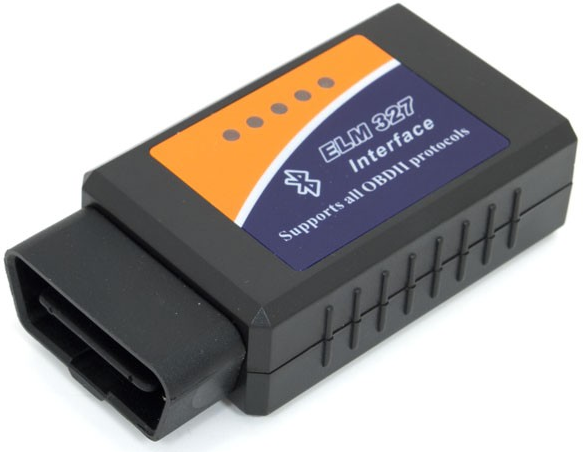
\includegraphics[width=2in]{img/elm_327_presentation}
  \caption{\textit{Elm 327} Bluetooth/OBDII module}
\end{figure}

By default, our module is discovered with the Bluetooth name "CHX" and requires the password "6789" for pairing.

\subsection{Connectors and Wirings}

The Flex Demo Board pins involved in the project are the following:

\begin{figure}[H]
  \centering
  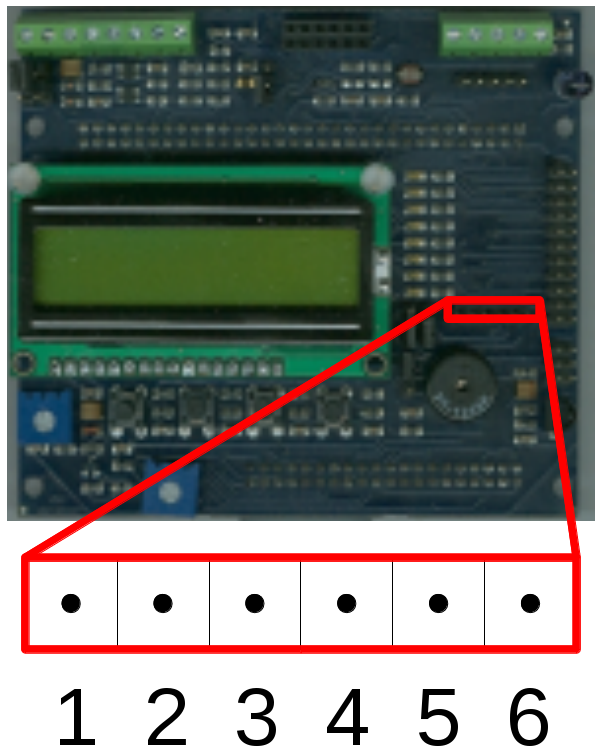
\includegraphics[width=2in]{img/flex_demo_board_pinout}
  \caption{\textit{Flex Demo Board} pinout}
\end{figure}

\begin{compactitem}
\item pin 1: 5 V;
\item pin 2: TX-O, UART output;
\item pin 3: SCK, Serial ClocK;
\item pin 4: RX-I, UART input;
\item pin 5: i.e. Vout;
\item pin 6: i.e. GND.
\end{compactitem}

The Bluetooth device uses has the following pinout:

\begin{figure}[H]
  \centering
  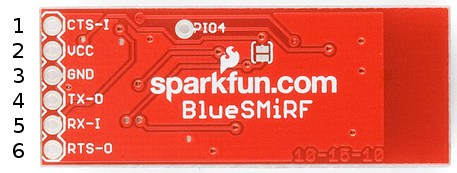
\includegraphics[width=3in]{img/bluesmirf_pinout}
  \caption{\textit{Bluesmirf} (Bluetooth/UART module) pinout}
\end{figure}

\begin{compactitem}
\item pin 1: CTS-I, Clear to Send (handshake pin);
\item pin 2: VCC (from 3.3V to 6V);
\item pin 3: GND;
\item pin 4: TX-O, UART output;
\item pin 5: RX-I, UART input;
\item pin 6: RTS-O, Request to Send (handshake pin).
\end{compactitem}

The Bluesmirf module has been connected to the Flex Demo Board with the following wiring:

\begin{compactitem}
\item Flex RX-I <-> Bt TX-O;
\item Flex TX-O <-> Bt RX-I;
\item Flex 5 V <-> Bt Vcc;
\item Flex GND <-> Bt GND.
\end{compactitem}

The standard OBDII female connector has the following pinout:

\begin{figure}[H]
  \centering
  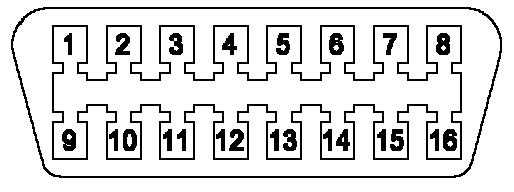
\includegraphics[width=2.5in]{img/J1962_female_pinout}
  \caption{OBD female connector pinout}
\end{figure}

\begin{compactitem}
\item pin 1: NC;
\item pin 2: Bus+ (J1850);
\item pin 3: NC;
\item pin 4: GND (chassis);
\item pin 5: GND (signal);
\item pin 6: CAN High (J-2284);
\item pin 7: K-Line (ISO9141-2);
\item pin 8: NC;
\item pin 9: NC;
\item pin 10: Bus (J1850);
\item pin 11: NC;
\item pin 12: NC;
\item pin 13: NC;
\item pin 14: CAN Low (J-2284);
\item pin 15: L-Line (ISO9141-2);
\item pin 16: Board Power (12 V).
\end{compactitem}


%------------------------------------------------

\section{Software}

\subsection{Elm327 Communication Basics}

Elm327 accepts basically two types of input:
\begin{compactitem}
  \item commands: allow various kind of operations on device;
  \item data requests: allow to retrieve data from the vehicle.
\end{compactitem}

Elm327 is case-insensitive and does not care about spacing symbols (tabs or white spaces).
Nevertheless, in this document will be used uppercases and a correct amount of spacing, with the aim of improving readability.

\subsubsection{Basic Commands}

All commands are prefixed with "AT". It is possible to distinguish between four classes of commands:
\begin{compactitem}
  \item general commands;
  \item OBD commands;
  \item protocols specific commands;
  \item miscellaneous commands.
\end{compactitem}

The syntax for commands is, usally
\begin{lstlisting}[language=bash]
AT CMD [param]
\end{lstlisting}

\begin{lstlisting}[language=bash]
AT Z
\end{lstlisting}

Resets the module, as if a power reset happened.
It brings back all the settings to their default values.

\begin{lstlisting}[language=bash]
AT SP x
\end{lstlisting}

Sets the protocol to \emph{x}, in particular, by default:
\begin{compactitem}
  \item 0 automatic;
  \item 1 SAE J1850 PWM (41.6 Kbaud);
  \item 2 SAE J1850 VPW (10.4 Kbaud);
  \item 3 ISO 9141-2 (5 baud init, 10.4 Kbaud);
  \item 4 ISO 14230-4 KWP (5 baud init, 10.4 Kbaud);
  \item 5 ISO 14230-4 KWP (fast init, 10.4 Kbaud);
  \item 6 ISO 15765-4 CAN (11 bit ID, 500 Kbaud);
  \item 7 ISO 15765-4 CAN (29 bit ID, 500 Kbaud);
  \item 8 ISO 15765-4 CAN (11 bit ID, 250 Kbaud);
  \item 9 ISO 15765-4 CAN (29 bit ID, 250 Kbaud);
  \item A SAE J1939 CAN (29 bit ID, 250* Kbaud);
  \item B USER1 CAN (11* bit ID, 125* Kbaud);
  \item C USER2 CAN (11* bit ID, 50* Kbaud).
\end{compactitem}

\subsubsection{Basic Data}

Each data request has three parameters associated:
\begin{compactitem}
  \item mode: hexadecimal 2 byte identifier;
  \item pid: hexadecimal 2 byte identifier;
  \item response length.
\end{compactitem}

Each request has the following syntax
\begin{lstlisting}[language=bash]
MODE PID
\end{lstlisting}
and each response has the syntax
\begin{lstlisting}[language=bash]
MODE PID VALUE
\end{lstlisting}
where \emph{VALUE} has different fixed sizes for different data.
\emph{VALUE}'s length is \emph{n}-byte, each one separated by a space symbol.

\begin{lstlisting}[language=bash]
01 01
\end{lstlisting}
Request the list of error codes (\emph{DTCs}, \emph{Diagnostic Trouble Codes}).
This returns a 4 byte response, like
\begin{lstlisting}[language=bash]
41 01 AA BB CC DD
\end{lstlisting}
where:
\begin{compactitem}
  \item \emph{41 01}: represents the response to the request;
  \item \emph{AA}: is the number of trouble codes:
  \begin{compactitem}
    \item most significant bit: Multifunction Indicator Lamp (MIL, aka Check Engine Light) has been turned on;
    \item remaining bits: number of stored trouble codes, flagged in the ECU (Engine Control Unit);
  \end{compactitem}
  \item \emph{BB CC DD}: information about the availability and completeness of certain on-board tests, with different interpretations in case of spark or compression ignition engines. More details on SAE J1979 documentation.
\end{compactitem}

So, with the \emph{AA} value set to \emph{81} hex (\emph{10000001} bin) it is possible to recognize that there is one trouble code stored which turned on the Check Engine Light.

\begin{table}[H]
\centering
\begin{tabular}{llr}
\multicolumn{3}{c}{BB} \\
\toprule
Test & Available & Incomplete \\
\midrule
Misfire & B0 & B4 \\          
Fuel System & B1 & B5 \\
Components & B2 & B6 \\
\bottomrule
\end{tabular}
\end{table}

\begin{table}[H]
\centering
\begin{tabular}{llr}
\multicolumn{3}{c}{CC, DD Spark Ignition} \\
\toprule
Test & Avail. & Incompl. \\
\midrule
Catalyst & C0 & D0 \\
Heated Catalyst & C1 & D1 \\
Evaporative System & C2 & D2 \\
Secondary Air System & C3 & D3 \\
A/C Refrigerant & C4 & D4 \\
Oxygen Sensor & C5 & D5 \\
Oxygen Sensor Heater & C6 & D6 \\
EGR System & C7 & D7 \\
\bottomrule
\end{tabular}
\end{table}

\begin{table}[H]
\centering
\begin{tabular}{llr}
\multicolumn{3}{c}{CC, DD Compression Ignition} \\
\toprule
Test & Avail. & Incompl. \\
\midrule
NMHC Cat & C0 & D0 \\
NOx/SCR Monitor & C1 & D1 \\
Boost Pressure & C3 & D3 \\
Exhaust Gas Sensor & C5 & D5 \\
PM filter monitoring & C6 & D6 \\
EGR and/or VVT System & C7 & D7 \\
\bottomrule
\end{tabular}
\end{table}




Response should be interpreted as a bit map.

\subsubsection{Communication Example}
We will use a fake Elm327 with a v1.5 firmware.
When connected, it is possible to launch the command
\begin{lstlisting}[language=bash]
AT Z
\end{lstlisting}

This command will reboot the module and print out the device name and firmware version
\begin{lstlisting}[language=bash]
ELM327 v1.5
\end{lstlisting}

\subsection{Linux/BlueZ}

It is necessary to add a new entry with the following format
\begin{lstlisting}[language=bash]
REMOTE PIN
\end{lstlisting}
to
\begin{lstlisting}[language=bash]
/var/lib/bluetooth/LOCAL/pincodes
\end{lstlisting}
where:
\begin{compactitem}
\item \emph{LOCAL} is the address of the Bluetooth device connected to PC;
\item \emph{REMOTE} is the address of the remote Bluetooth device (in our case, the Elm327 interface);
\item \emph{PIN} is the pin code used by the remote Bluetooth device for pairing.
\end{compactitem}

\begin{table}[H]
\caption{Example table}
\centering
\begin{tabular}{llr}
\toprule
\multicolumn{2}{c}{Name} \\
\cmidrule(r){1-2}
First name & Last Name & Grade \\
\midrule
John & Doe & $7.5$ \\
Richard & Miles & $2$ \\
\bottomrule
\end{tabular}
\end{table}

\lipsum[5] % Dummy text

\begin{equation}
\label{eq:emc}
e = mc^2
\end{equation}

\lipsum[6] % Dummy text

%------------------------------------------------

\section{Manual}

%\lipsum[7-8] % Dummy text
\subsection{Wiring}

Wire the module like that.

\subsection{User Interaction}

Software starts with a welcome message...


%----------------------------------------------------------------------------------------
%	REFERENCE LIST
%----------------------------------------------------------------------------------------

\begin{thebibliography}{99} % Bibliography - this is intentionally simple in this template

\bibitem{} A. S. Huang, L. Rudolph,
  \emph{Bluetooth Essentials for Programmers},
  Cambridge University Press (2007)

\bibitem{}
  \emph{Bluetooth Data Module Command Reference \& Advanced Information User's Guide},
  Roving Networks (2013)
  
\bibitem{}
  \emph{ELM327 - OBD to RS232 Interpreter},
  Elm Electronics
 
\end{thebibliography}

%----------------------------------------------------------------------------------------

\end{multicols}

\end{document}
